\section{Mechanizm budowania oraz zarządzanie zasobami w grach RTS (Bogna Lew)}\label{s:budowanie}
Jednym z typowych elementów gier strategii czasu rzeczywistego  jest tworzenie baz i budowanie fortyfikacji. Mechanizm
ten stanowi urozmaicenie rozgrywki i wprowadza dodatkowe aspekty możliwe do uwzględnienia w planowaniu strategii. Dla
wielu gier RTS jest wręcz nieodłącznym elementem, który umożliwia graczowi tworzenie i rozwój nowych jednostek,
produkcję zasobów, umacnianie swojej pozycji oraz zwiększanie swojej potęgi.

Mechanizm ten wiąże się z szeregiem ograniczeń, które mają kluczowy wpływ na rozgrywkę. Należą do nich między innymi
ograniczenia związane z ukształtowaniem terenu oraz obecnością innych elementów scenerii. Każde z tych ograniczeń ma
swoje źródło w prawdziwym świecie i mechanizm budowania musi je uwzględniać.

Z tą mechaniką związany jest system zasobów, który jest popularnym aspektem gier z tego gatunku. Wiele gier strategii
czasu rzeczywistego umożliwia graczowi budowanie własnej ekonomii. Uzyskane przez niego zasoby często mogą zostać
wykorzystane przez mechanizm budowania jako koszta budowy obiektów.

Przykładem gry strategii czasu rzeczywistego implementującej tę mechanikę jest \textit{Warhammer 40,000: Dawn of War}\footnote{\url{https://www.dawnofwar.com/}}. Jest to
gra, której realia są osadzone w uniwersum gry bitewnej \textit{Warhammer 40,000}. Udostępnia ona tryb jednoosobowy oraz
wieloosobowy dla maksymalnie sześciu graczy. W pierwszym wariancie gracz wciela się w postać dowódcy
armii Space Marines z Blood Ravens i ma za zadanie zapobiec inwazji Orków. Gra \textit{Warhammer 40,000: Dawn of War} bardzo szybko
zyskała na popularności i oferowała wszystko, co było potrzebne dla tego gatunku. Z tego powodu warto się jej przyjrzeć,
pomimo faktu, że jej realia znacząco odbiegających od tych, w których zostanie osadzona tworzona przez nas gra.

\textit{Warhammer 40,000: Dawn of War} wyróżnia model pozyskiwania surowców. W grze dostępne są dwa rodzaje: Energia, która jest
generowana przez dedykowane do tego budowle oraz Rekwizycja, której szybkość wytwarzania jest uzależniona od kontrolowanych
przez gracza punktów strategicznych. Taka mechanika znacznie lepiej wpasowuje się w realia gry oraz wymusza na użytkowniku
przyjęcie agresywniejszej strategii.

Dodatkowo \textit{Warhammer 40,000: Dawn of War} posiada typowy dla gier RTS mechanizm tworzenia budowli. Gracz ma
do dyspozycji jednostki, którym może zlecić budowę wybranego przez siebie obiektu po poniesieniu kosztów jego utworzenia.
Zanim będzie możliwe rozpoczęcie budowania użytkownik musi wybrać miejsce, w którym budynek powstanie, co robi, przesuwając
jego podgląd po mapie. W tym czasie gra dokonuje walidacji miejsca i informuje gracza czy wybrany obszar jest poprawny,
odpowiednio podświetlając widok budynku. Wybudowanie obiektu nie jest natychmiastowe, co sprawia, że gra lepiej oddaje
realia, w których jest osadzona.

\begin{figure}[h!]
    \centering
    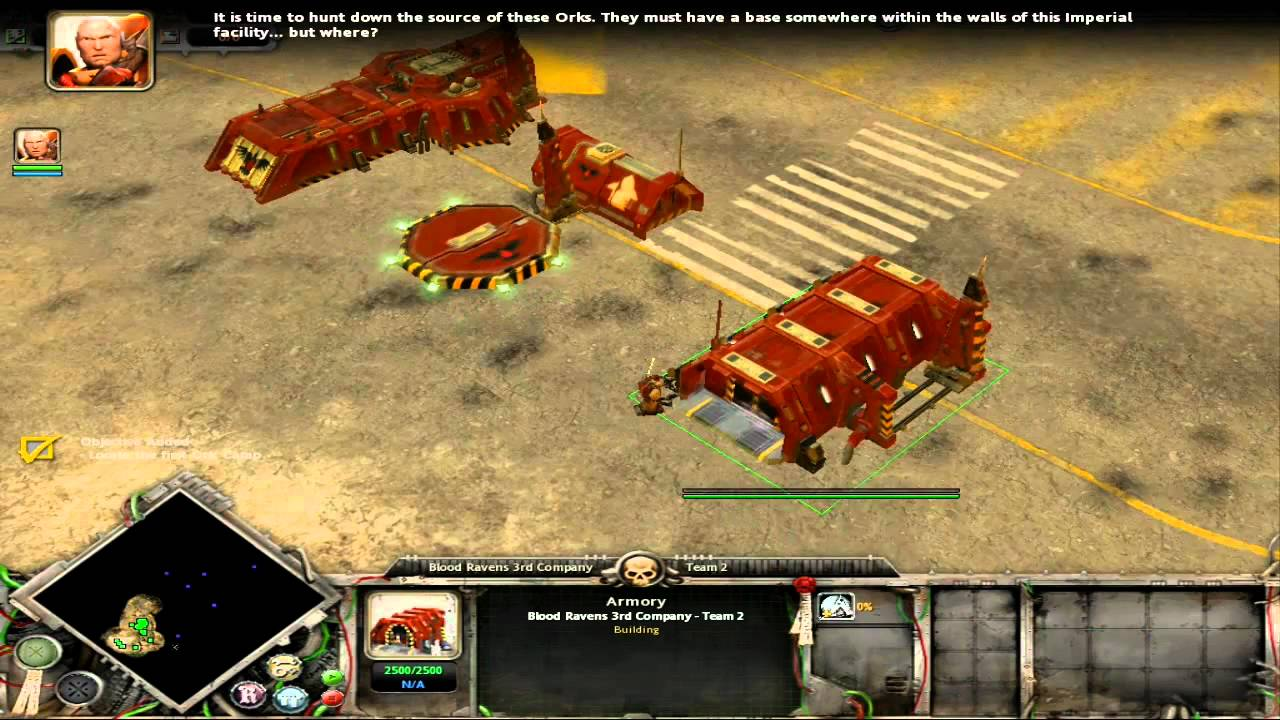
\includegraphics[width=0.9\textwidth]{images/warhammer1.jpg}
    \caption[Budowanie budynku przez dedykowaną do tego jednostkę w grze \textit{Warhammer 40,000: Dawn of War}.]{Budowanie budynku przez dedykowaną do tego jednostkę w grze \textit{Warhammer 40,000: Dawn of War}.\protect\footnotemark}
\end{figure}
\FloatBarrier
\footnotetext{Internet, \url{https://www.youtube.com/watch?v=wNtnGFoVReU}, dostęp: 19.11.2023}